\lab{Filtering and Convolution}{Filtering and Convolution}
\objective{ The Fourier transform reveals information in the frequency domain about signals and images that might not be apparent in the time (sound) or spatial domain (image). It provides an extremely powerful tool to analyze difficult problems simply. In this lab, we learn how to  use the Fourier transform to effectively convolve sound signals and filter out unwanted noise. } 

\section*{Convolution} % ========================================

Mixing two sounds signals is a common method used in signal processing and analysis. 
This is done through a discrete \emph{convolution}. 
% Recall that sound is modeled with discrete samples of a sound wave in rapid succession. 
Given two periodic sound samples $f$ and $g$ of length $n$, the convolution of these two samples is an $n$-dimensional vector where the $k$th component is given by
\begin{equation}
(f \ast g)_k = \sum_{j=1}^{n-1} f_{k-j}g_j,\,\,\,\,\,\,\,\,\,\,\,\,\,k = 0,1,2,\dots,n-1. % There must be a better way to make spaces here. 
\label{eq:naive-convolve}
\end{equation}

Since audio needs to be sampled frequently to create smooth playback, a recording of a song can contain tens of millions of samples. 
For example, a signal that is one minute long would have $2646000$ samples if the signal was sampled at $44100$ per second (which is the standard rate).
Therefore, convolving samples using the na\"ive method of convolution (\ref{eq:naive-convolve}) is very computationally expensive and often infeasible. 

Fortunately, the Fourier transform can calculate convolutions quickly. 
The Convolution Theorem states that 

\begin{equation}
\mathcal{F}(f \ast g) = \mathcal{F}(f)\cdot\mathcal{F}(g), 
\end{equation}

where $\mathcal{F}$ is the discrete Fourier transform, $\ast$ is convolution, and $\cdot$ is component-wise multiplication.
Thus, the convolution of two arrays is 

\begin{equation}
f \ast g = \mathcal{F}^{-1}(\mathcal{F}(f)\cdot\mathcal{F}(g)),
\end{equation}

where  $\mathcal{F}^{-1}$ is the inverse discrete Fourier transform. 

Recall that although the samples used are real numbers, taking the inverse Fourier transform of the samples may have small complex components due to rounding errors. 
To avoid this error, remember to take the real part of the inverse Fourier transform.

\begin{comment} % This will be explained in the first fourier lab.  
\begin{lstlisting}
# Example of complex rounding error when using the fft and ifft. 
>>> x = np.array([1,2,3,4,5,6])
>>> y = sp.ifft(sp.fft(a)) 
#Result is close to x but complex components are present due to rounding error. 
>>> y                       
array([ 1. +0.00000000e+00j,  2. -1.11022302e-15j,  3. +1.69171391e-15j,
        4. +1.71752100e-17j,  5. -3.59446285e-16j,  6. -2.39219815e-16j])
# Take the real part to get the desired result. 
>>> np.real(y)              
array([ 1.,  2.,  3.,  4.,  5.,  6.])
\end{lstlisting}
\end{comment} 

\subsection*{Circular Convolution}
The Convolution Theorem requires that the samples be periodic in the time domain. 
Due to the mathematical properties of the Fourier transform, the result of this convolution is a \emph{circular convolution}. 
This means that the convolution is assumed to be periodic and the sounds at the end of the signal will tend to mix with sounds at the beginning of the signal. 
A circular convolution creates an interesting effect on a signal when convoluted with a segment of white noise; the sound will loop seamlessly from the end back to the beginning.

\begin{comment}
\begin{problem} % White noise Problem. Currently commented out. 
Create white noise and listen to the resulting sound (\textbf{CAUTION:} Turn your volume \emph{way} down! It may be very, \emph{very} loud).
This kind of noise is called ``white" because it contains all frequencies with the same strength, or rather, with the same expected strength (since the amplitude of a specific frequency is a matter of chance).
In order to see this, plot the spectrum of the noise.
\end{problem}
\end{comment}

\begin{problem} % Circular convolution problem. 
Use SciPy's \li{sp.fft()} and \li{sp.ifft()} to create a \li{SoundWave} object that is the circular convolution of \texttt{tada.wav} with two seconds of white noise.
Note that the length of the two samples must be the same, so pad an array of zeros to the end of the \texttt{tada.wav} sample to match the length of the noise. 
You may use \li{np.append()} to add an array of zeros to the end of a sample. 

Make a sample of white noise by using NumPy's \li{random} module:
\begin{lstlisting}
# Create 2 seconds of mono white noise.
samplerate = 22050
noise = np.int16(np.random.randint(-32767, 32767, samplerate*2))
\end{lstlisting} 

To test your result, use the \li{append()} method in the \li{SoundWave} class to add multiple copies of the signal consecutively. 
Your new signal should have a continuous, seamless transition. 
\end{problem}

\subsection*{Linear Convolution}
Although circular convolution can have unique results, common mixtures of sounds do not have sound at the beginning of a signal to mix with the sound at the end of the signal. 
This form of convolution is called a \emph{linear convolution}.
The linear convolution of two samples with lengths $N$ and $M$ has length $N+M-1$. 
The simplest way to achieve this length when using the Convolution Theorem is to pad zeros at the end of both of the samples to have at least lengths $N+M-1$ and return only the first $N+M-1$ samples of the convolution. 

\begin{problem}
Write a function that accepts two arrays of sound samples and returns the linear convolution of the samples using the Fourier transform. 
Make sure to pad the right amount of zeros to the end of both samples to avoid circular convolution and return the correct length of sample. 

Print out and compare the time it takes to compute the convolution of the signals of \texttt{AEA.wav} and \texttt{EAE.wav} using the method you have written with SciPy's \li{sp.signal.fftconvolve()} function and a naive convolution function using Equation (\ref{eq:naive-convolve}) given below.  
 
\begin{lstlisting}
def naive_convolve(sample1,sample2):
    sig1 = np.append(sample1, np.zeros(len(sample2)-1))
    sig2 = np.append(sample2, np.zeros(len(sample1)-1))
    
    final = np.zeros_like(sig1)
    rsig1 = sig1[::-1]
    for k in range(len(sig1)-1):
        final[i+1] = np.sum((np.append(rsig1[i:],rsig1[::-i][:i]))*sig2)
    return final    
\end{lstlisting}

To test the convolution method, listen to the signal created with the fast Fourier transformation convolution. 
Compare your audio with the convolution created with SciPy's \li{signal.fftconvolve()}.  
\end{problem}

Suppose there is a recording of a musical piece played in a small, carpeted room with essentially no acoustics (little or no echo). 
The discrete linear convolution can mix this signal with an echoing sound to make the piece sound like it were played in a large concert hall with echo. 

When a balloon is popped in a large room with echo, the sound resonate in the room for up to several seconds.
This echoing sound is referred to as the \emph{impulse response} of the room, and is a way of approximating the acoustics of a room.
When the individual sounds of an instrument in a carpeted room is convoluted with the impulse response from a concert hall, the new signal will sound as if the instrument is being played in the concert hall.

\begin{comment}
% Random comments about the balloon convolution that was taken out. 
The first step recording of how a echoic room responds to a short pulse of sound.
Effective ways of producing a loud sound approximating a pulse--other than creating an actual pulse with a computer--include firing a (preferably blank) gunshot, popping a balloon, or, if neither of those options are available, clapping the hands one time.

The key is to recognize that this process can be described as a convolution: namely, the final sound is simply the convolution of the our original sound with the impulse response.
In other words, it is the original sound with the echoes of the prexious $n$ samples, where $n$ is the number of samples in the impulse response.

When these sounds are played back, the ear percieves them as a continuous soundwave.
In other words, sound playback is a series of pulses of varying intensities, similar to the pulse in an impulse response.
If we ``mix'' the individual sounds of an instrument in a carpeted room with the impulse response from a concert hall, then the new soundwave will sound as if the instrument is being played in the concert hall.
This ``mixing'' is better referred to as \emph{convolution}. With the impulse response, we can see how sound echoes and decays.  This ``echoicness'' can then be combined with each audio sample to reproduce the echo at the appropriate time and amplitude.
Each of these samples needs to be combined with the impulse response, which may be several seconds long.
\end{comment}

\begin{comment}
% Recording problem is now deleted. 
\begin{problem}
(Optional)\footnote{If the instructor does not require this problem then students may use the provided \texttt{balloon.wav} file which contains the sound of a balloon pop in a large room.} Find a large room or area with good acoustics, and record (an approximation to) its impulse response using a balloon pop.
To record the sound, you will want to use at least a decent microphone.
You may want to record it using the program Audacity\footnote{Audacity is free sound manipulation software and may be downloaded at http://audacity.sourceforge.net} and a laptop.
If you use a unidirectional microphone, be sure the microphone is pointing at the balloon when you pop it, so that the direct sound from the pop is picked up.
(If you don't, the result will still be okay.
However, after the convolution it will probably sound somewhat distant, as if we were standing somewhere where we couldn't hear the music directly.)
If you've chosen a good room, the response should be audible for at least a full second.
Include a plot of both the waveform and spectrum of the impulse response you recorded.
\end{problem}
\end{comment}

% Convolve the balloon pop with Chopin.
\begin{problem}
The \texttt{chopin.wav} file is a signal with piano being played in a dead room with little or no acoustics, and the \texttt{balloon.wav} file is a recording of a balloon pop in an echoic room. 
Use SciPy's \li{signal.fftconvolve()} to take the convolution of \texttt{chopin.wav} with \texttt{balloon.wav}.

Listen to the new signal, there should be echo in the piano recording. 
\begin{comment}
To summarize:
\begin{enumerate}
\item Read in \texttt{chopin.wav} and the impulse response with \li{wavfile},
\item Add several seconds of silence to the signal from \texttt{chopin.wav},
\item Insert zeros into the middle of the impulse response transform so that it is the same length as  \texttt{chopin.wav},
\item Calculate the convolution of the signals,
\item And finally, calculate the inverse Fourier transform.
\end{enumerate}
\end{comment}
\end{problem}

% Old problem exploring Stereo vs. Mono.
\begin{comment}
\begin{problem}
Record yourself singing a few notes (or, feel free to produce some other sound another way).
Take the circular convolution of white noise with this recording.
Now do it again using stereo white noise.
This is just like the mono white noise problem, but make the NumPy array in two dimensions.
It's no problem that your original recording will probably be mono; just make the left and right channels duplicate in the recording (but be sure to use different left and right channels for the white noise).
Can you hear any difference between the mono and stereo versions of the result?
\end{problem}

Feel free to play around with this. The file \texttt{guitar-conv.mp3} is a collage of sounds created using this technique (mostly using guitar samples).
\end{comment}

\begin{figure}[H]
\captionsetup[subfigure]{justification=centering}
\centering
\begin{subfigure}{.5\textwidth}
    \centering
    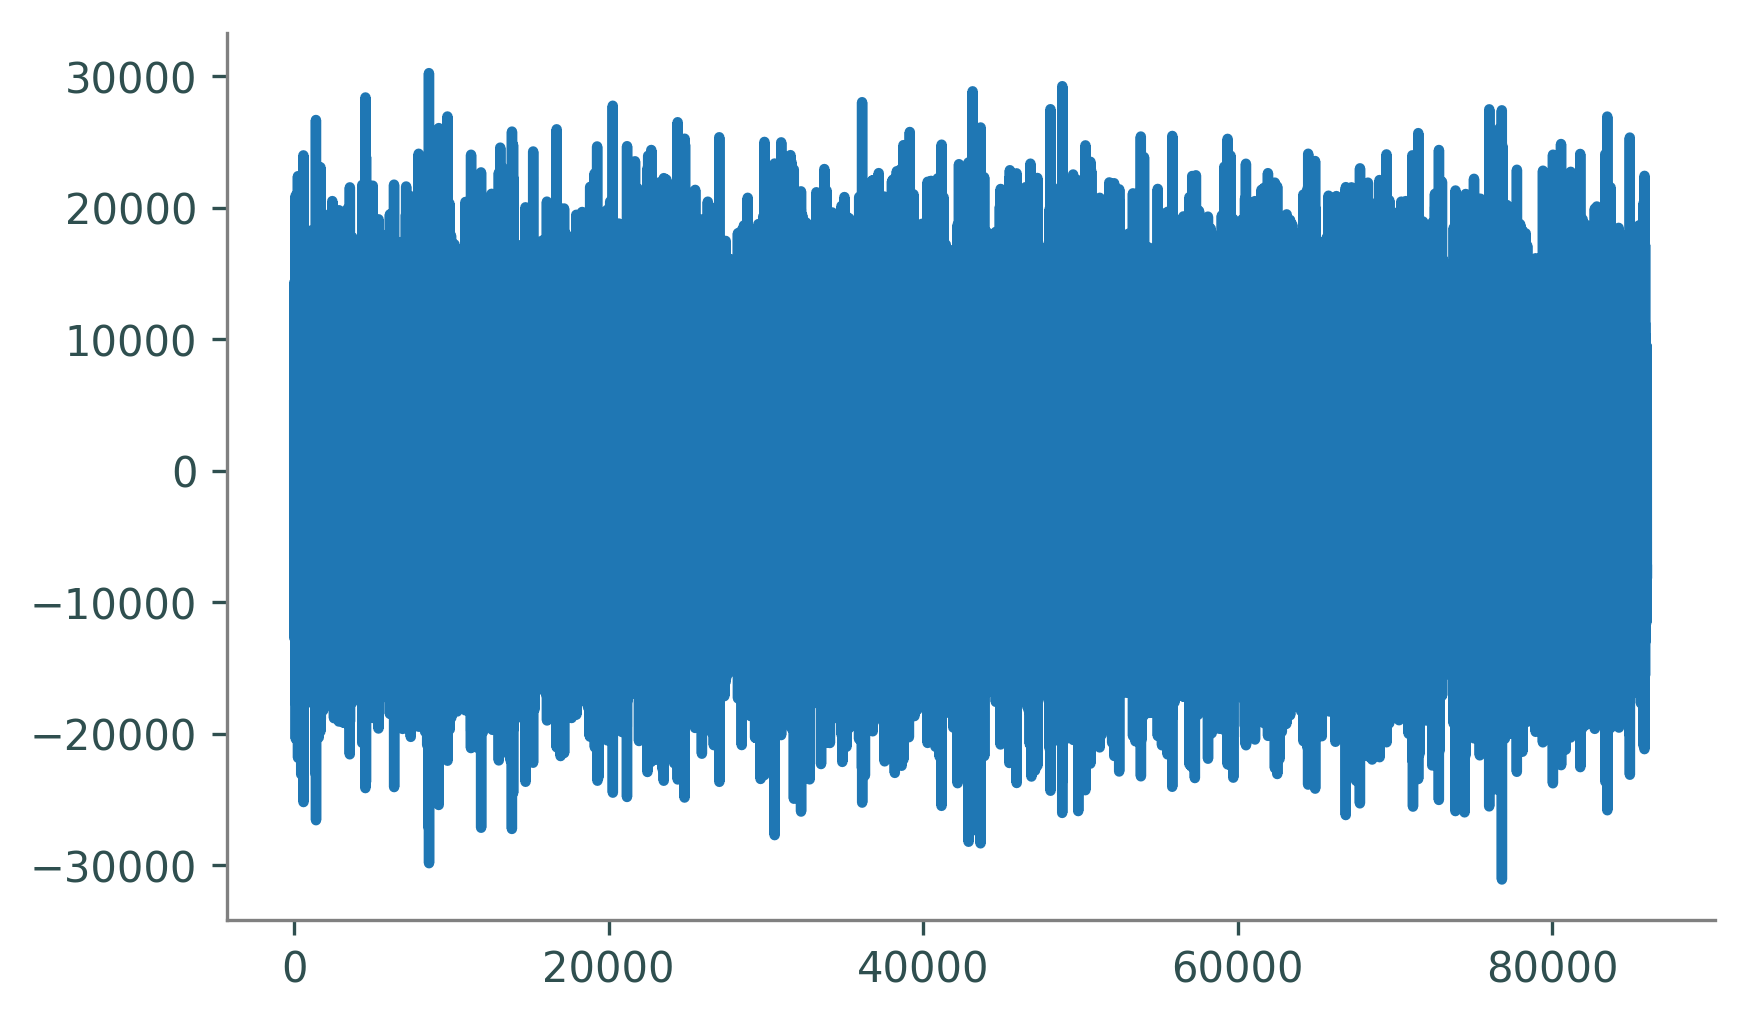
\includegraphics[width=\linewidth]{figures/noisy.png}
    \caption{Signal in the time domain.}
    \label{fig:noisysignal}
\end{subfigure}%
\begin{subfigure}{.5\textwidth}
    \centering
    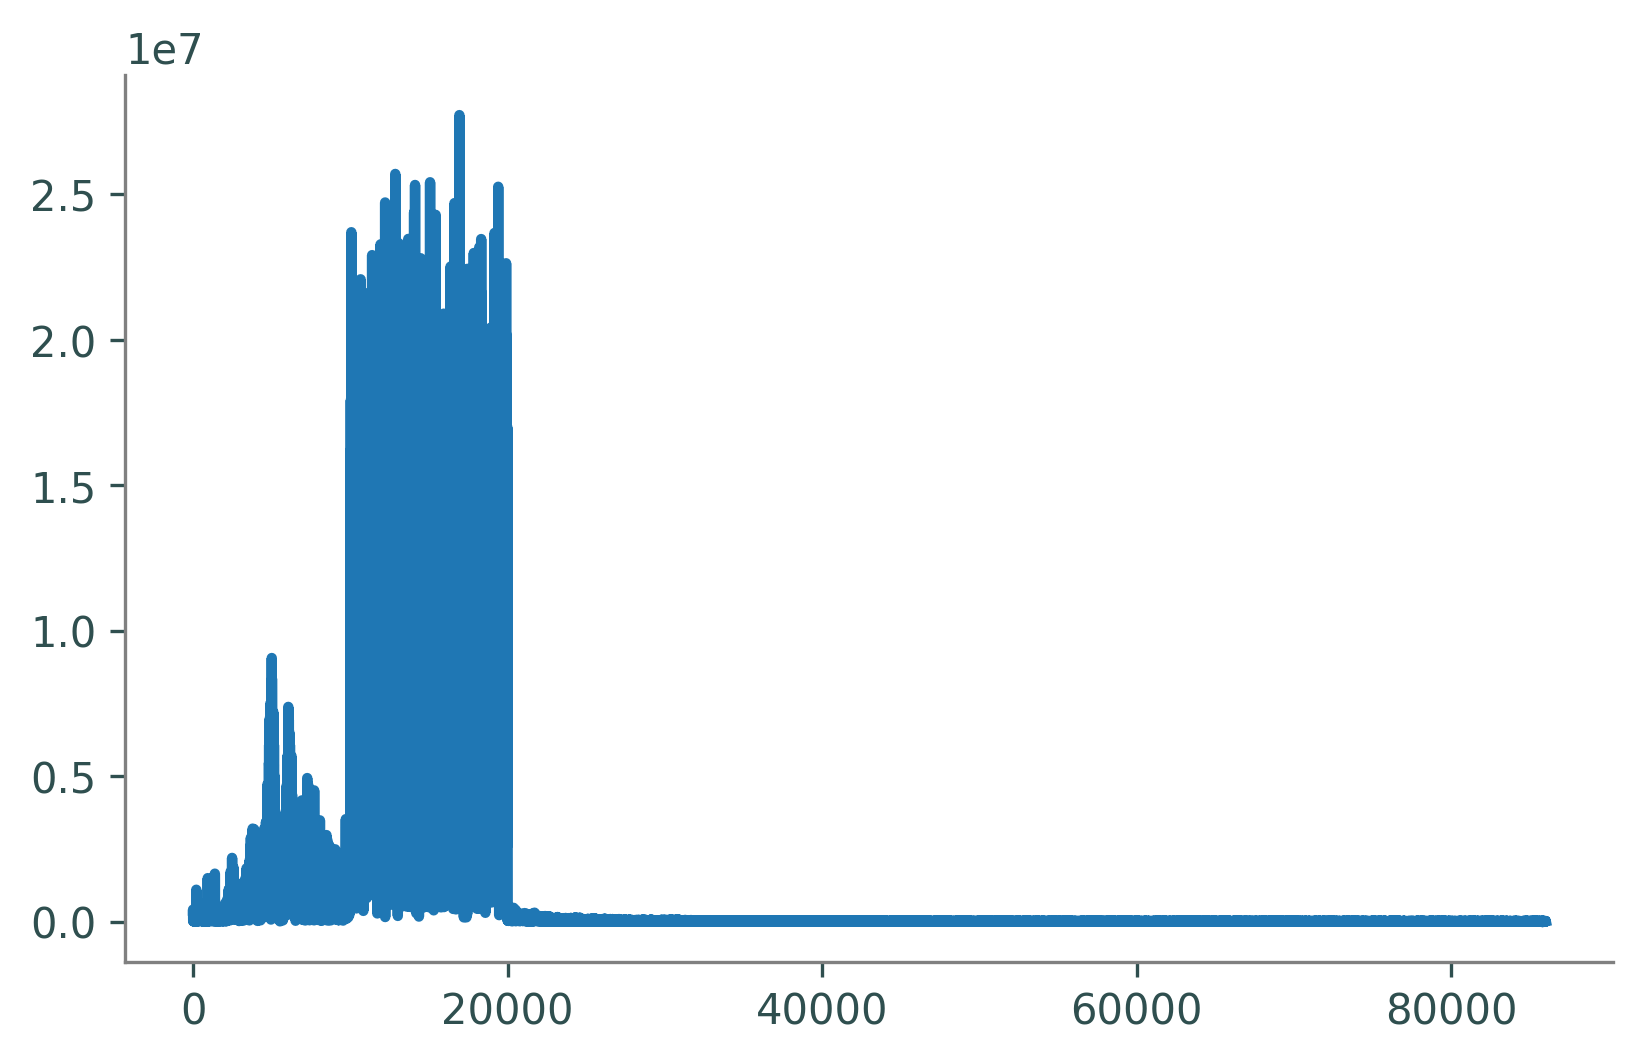
\includegraphics[width=\linewidth]{figures/noisyspec.png}
    \caption{Signal in the frequency domain.}
    \label{fig:noisyspec}
\end{subfigure}
\caption{The \texttt{Noisysignal1.wav} signal}
\end{figure}

\section*{Cleaning up Noise} % =======================================

The Fourier transform also reveals important information about images and signals in the frequency domain. 
For example, Figure \ref{fig:noisysignal} plots a noisy recording of a voice over time. 
This plot has a lot of static and does not reveal a lot of information about the signal. 

The Fourier transform of the signal in Figure \ref{fig:noisyspec}, however, reveals that the static in the time domain is the result of some concentrated noise between $1250$ Hz to  $2500$ Hz. 
Remove this noise at those frequencies to remove the noise of the signal.

Recall that the plot of a signal in the frequency domain is the plot of the discrete Fourier transform (DFT) with the x-axis scaled to reveal the amplitude at each frequency. 
This was done by multiplying the domain of the DFT by the sampling rate and dividing by the number of samples in the signal. 

Hence, to remove the high amplitudes at certain frequencies between between $1250$ to $2500$ Hz in the signal, find the indices of the DFT array that correspond to those frequencies and set them to zero. 
In order to find the correct indices of the DFT array corresponding to these frequencies, multiply the frequency by the number of samples and dividing by the sampling rate. 
Make sure that the index is an integer. 

\begin{lstlisting}
# Find the indices of the DFT that corresponds with the frequencies 1250 and 2500.
>>> low = 1250*len(samples)//rate
>>> high = 2500*len(samples)//rate
\end{lstlisting}

The plot in Figure \ref{fig:noisyspec} has also been cut in half since the DFT is symmetric. 
Therefore, if the coefficient at index $j$ is set to $0$, then the coefficient at index $N - j$  must be set to $0$ as well, where $N$ is the number of discrete Fourier samples.

\begin{lstlisting}
# Set the chosen coefficients between low and high to 0.
>>> fft_sig[low:high]=0
>>> fft_sig[-high:-low]=0
\end{lstlisting}

Then calculate the inverse Fourier transform to get a new, clean signal.

The plot of this new signal in the time domain now reveals individual syllables as they are spoken.
See Figure \ref{fig:cleansignal}. % Fix image and add new image. 

\begin{figure}[H]
    \centering
    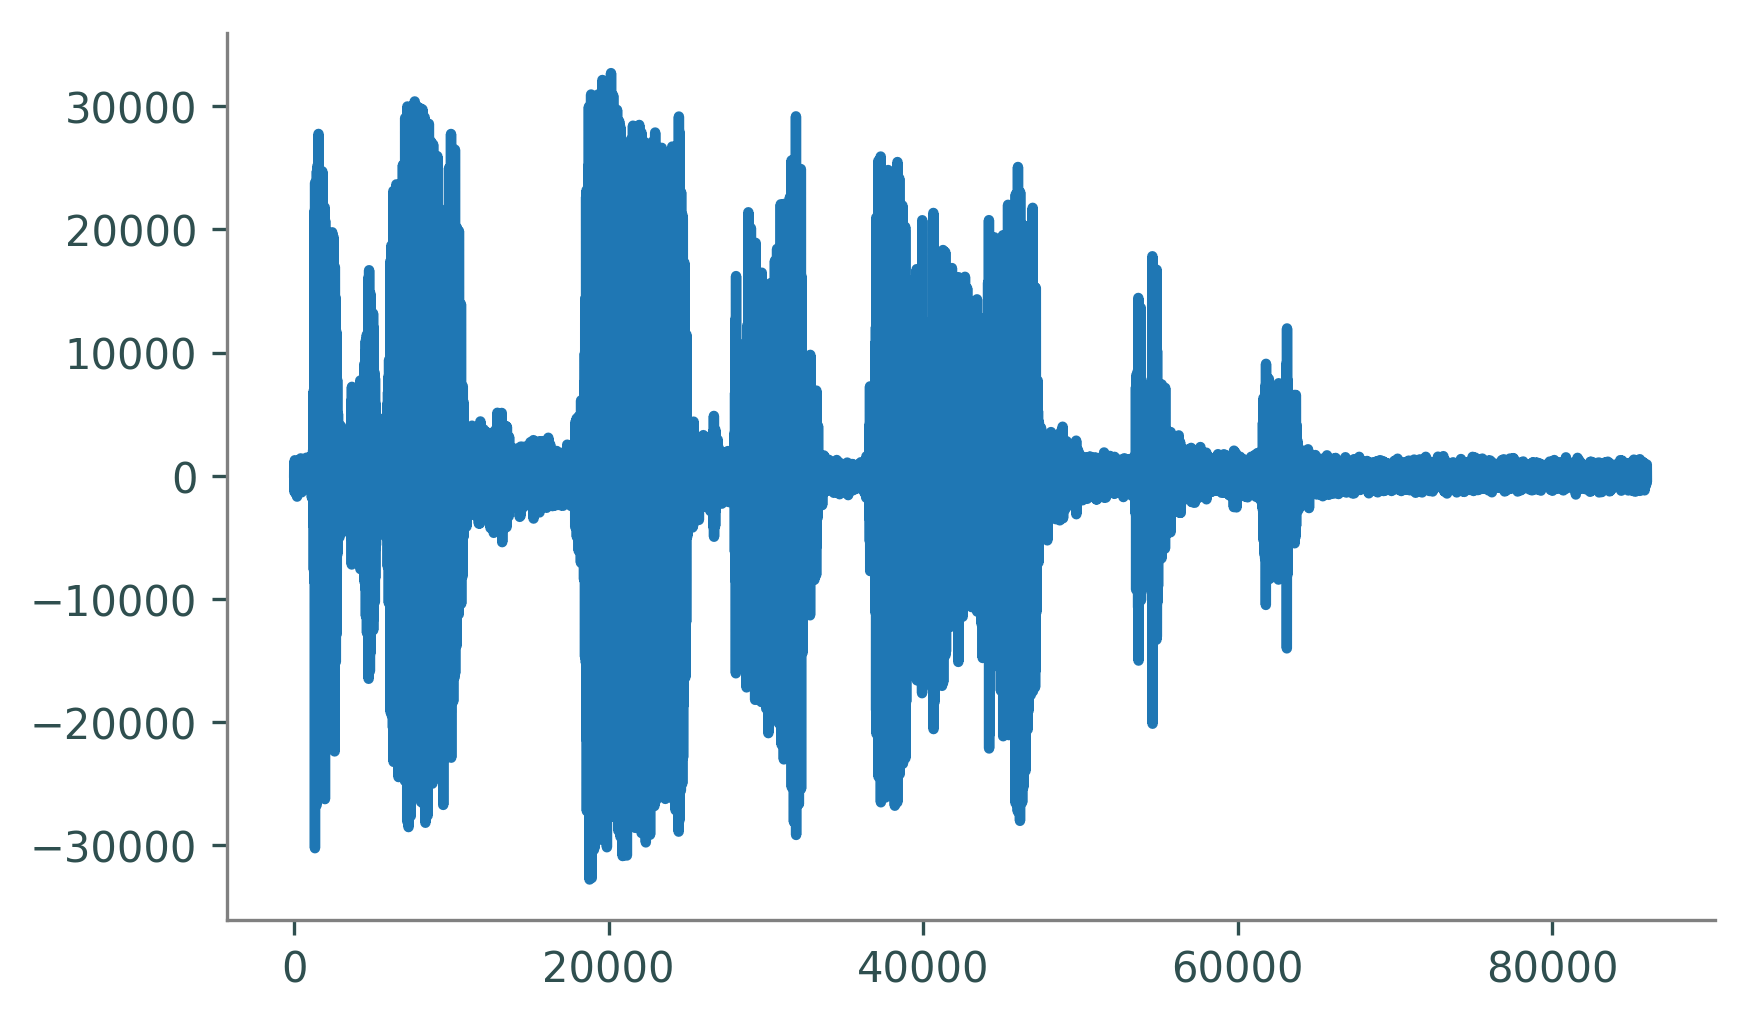
\includegraphics[width=.7\textwidth]{figures/Cleanedsignal.png}
    \caption{The plot of \texttt{Noisysignal1.wav} in the time domain after being cleaned.}
    \label{fig:cleansignal}
\end{figure}

\begin{problem} % Clean up a noisy signal (The only thing we have to fear...)
Write a function that accepts a sound sample, a sample rate and low and high frequencies that define a range of frequencies to remove using the technique described above. 
It should return an array of samples that has the indicated frequencies removed. 

Listen to \texttt{Noisysignal2.wav}, which just sounds like random noise. 
Use the \li{SoundWave} class to plot the discrete Fourier transform of this signal to see at what frequencies is the noise present. 
Remove the noise using the function you have written and create a \li{SoundWave} object from the new signal. 

It may be helpful to plot the DFT of the new signal to fine-tune the low and high frequencies chosen to filter out. 

Listen to the filtered signal and see if you can recognize the famous person speaking. 
\end{problem}

When a digital audio signal is played on a computer, the signal is sent to a speaker, which vibrates, producing sound waves.  
When multiple speakers are used, they can all produce the same signal or they can produce different signal. 
When there is only one signal, the sound is \emph{monoaural}, or \emph{mono}.  When speakers produce more than one signal, the overall signal is \emph{stereophonic}, or \emph{stereo}.  Usually stereo means two, but there may be any number of signals ($5.1$ surround sound, for instance, has $5$). 

All of the sounds used in this lab so far were mono; hence, the samples were only one dimensional arrays. 
More commonly, signals are multi-dimensional, and can be treated similarly to mono signals.  

\begin{problem}
During the 2010 World Cup in South Africa, large plastic horns called vuvuzelas were blown excessively throughout the games.
Broadcasting organizations faced difficulties with their programs due to the noise level of these vuvuzelas. 
To solve this problem, audio filtering techniques were used to cancel out the sound of the vuvuzela which has a frequency of around 200-500 Hz. 

Listen to \li{vuvuzela.wav}\footnote{A clip of \url{https://www.youtube.com/watch?v=g_0NoBKWCT8}.} and notice the low humming sound of the vuvuzelas in the background.  
Use the function written previously to create a new \li{SoundWave} object that removed the vuvuzela noise. 
Note that the sound file is a stereo sound with two sound signals. 
The first and second column of the array sample corresponds to the signals for the left and right speaker respectively.  
Filter out the frequencies of the vuvuzela in each signal. 
Then combine the two samples back to its original form. 

Listen to the resulted signal to see whether the vuvuzela horns has successfully been filtered out. 

\end{problem} 

\subsection*{The 2-Dimensional FFT}

The Fourier transform can be readily extended to any number of dimensions. 
Computationally, the problem reduces to performing the one-dimensional Fourier transform iteratively along each of the dimensions.
This lab focuses only on the Fourier transform of two-dimensional matrices.
The Fourier transform of two-dimensional matrices is useful for image denoising, image compression, edge-detection, image enhancement, and more.

Given a matrix $A$, first calculate the one-dimensional Fourier transform of each column, storing the result column-wise in an array the same shape as $A$.
Then calculate the Fourier transform of each row of this resulting array.
This yields the two-dimensional Fourier transform of $A$.
Calculating the two-dimensional inverse Fourier transform is done in a similar fashion, but in the opposite order: first calculate the inverse Fourier transform of the rows, then the columns. 

The NumPy module has functions that perform these operations.

\begin{lstlisting}
>>> A = np.array([[5, 3, 1], [4, 2, 7], [8, 9, 3]])
# Calculate the Fourier transform of A.
>>> fft = np.fft.fft2(A)
# Calculate the inverse Fourier transform.
>>> ifft = np.fft.ifft2(fft)
>>> np.allclose(A, ifft)
True
\end{lstlisting}

\subsection*{Images}

Just as the one-dimensional Fourier transform can be used to remove noise in sounds, its two-dimensional counterpart can be used to remove noise in images.
By taking the two-dimensional Fourier transform of a noisy, or blurry, image as described above, we can determine the frequencies that are causing the blur and alter them. 
Taking the inverse Fourier transform of this produces a less-blurry version of the original image.
Note that in order for this process to work perfectly, the noise must be periodic and all problem areas in the Fourier transform must be changed correctly.
As a result, it is very difficult to completely remove all noise from an image using only the Fourier transform, but depending on the situation, it may be capable of removing enough noise to be useful.

\begin{figure}
\captionsetup[subfigure]{justification=centering}
\centering
\begin{subfigure}{.4\textwidth}
    \centering
    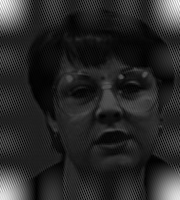
\includegraphics[width=\linewidth]{figures/blurry_face.png}
    \caption{The original blurry image.}
    \label{fig:blurry_face}
\end{subfigure}
\begin{subfigure}{.4\textwidth}
    \centering
    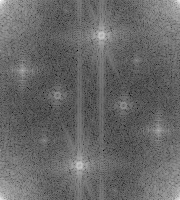
\includegraphics[width=\linewidth]{figures/blurry_fft.png}
    \caption{The FFT of the original image.}
    \label{fig:blurry_fft}
\end{subfigure}
\begin{subfigure}{.4\textwidth}
    \centering
    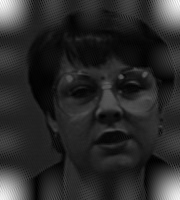
\includegraphics[width=\linewidth]{figures/improved_face.png}
    \caption{The improved image.}
    \label{fig:covered_fft}
\end{subfigure}
\begin{subfigure}{.4\textwidth}
    \centering
    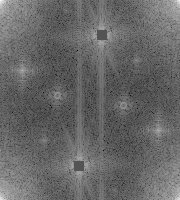
\includegraphics[width=\linewidth]{figures/covered_fft.png}
    \caption{The FFT of the improved image.}
    \label{fig:improved_face}
\end{subfigure}
\label{fig:image_fft}
\caption{To remove noise from an image, take the Fourier transform of the image and replace the abnormalities with values more consistent with the rest of the FFT. 
Notice that the new image is less noisy, but only slightly.
This is because only some of the abnormalities in the FFT were changed.
In order to further decrease the noise, we would need to further alter the FFT.}
\end{figure}

Below is an example of how this process works.
The following code refers to figure \ref{fig:image_fft}.
First plot the original blurry image.

\begin{lstlisting}
# Plot the blurry image (figure 1.3(a)).
>>> from scipy.misc import imread
>>> image = imread("face.png", True)
>>> plt.imshow(image, cmap='gray')
>>> plt.show()
\end{lstlisting}

Now plot the Fourier transform of this image in order to see where the spikes in frequency are.
To effectively visualize this plot, plot the log of the absolute value of the result.

\begin{lstlisting}
# Plot the Fourier transform of the blurry image (figure 1.3(b)).
>>> fft = np.fft.fft2(image)
>>> plt.imshow(np.log(np.abs(fft)), cmap='gray')
>>> plt.show()
\end{lstlisting}

Notice the spikes in the plot.
In order to reduce the noise in the plot, replace these abnormally high values with values that are more similar to those around them.
There are many ways to do this, but one possibility is to simply "patch" it by covering the area with a small matrix of values similar to other values in the plot.

\begin{lstlisting}
# Cover the spikes in the Fourier transform (figure 1.3(d)).
>>> fft[30:40, 97:107] = np.ones((10,10)) * fft[33][50]
>>> fft[-39:-29, -106:-96] = np.ones((10,10)) * fft[33][50]
>>> plt.imshow(np.log(np.abs(fft)),cmap='gray')
>>> plt.show()
\end{lstlisting}

Finally, take the inverse Fourier transform of this to get an image similar to the original, but with less noise.
Notice that this new image still has noise present, but is less noisy than the original.
Once again, use the absolute value of this result to plot it.

\begin{lstlisting}
# Plot the new image (figure 1.3(c)).
>>> new_image = np.abs(np.fft.ifft2(fft))
>>> plt.imshow(new_image, cmap='gray')
>>> plt.show()
\end{lstlisting}

In practice, it often will suffice to remove some of the noise, even if it is not possible to remove all of it.
For example, if the purpose of cleaning up an image was to retrieve some information from it that was not easily distinguishable before, then it would be sufficient to only remove enough noise to accurately extract that information.
To further improve the image, a similar process to the one described above must be done to cover the remaining spikes.

\begin{problem}
One potential application of removing noise from an image is cleaning up an image of a license plate to retrieve its information. 
The file \li{license_plate.png} contains a blurred image of a license plate. 
In the bottom right corner of this image, there is a sticker that has information about the month and year that the license plate was renewed. 
However, in its current state the year is not clearly legible.
Use the two-dimensional Fourier transform to clean up the image enough that the year in the bottom right corner is legible. 
\end{problem}





\begin{comment}

\section*{Image Filters} % ====================================================

Recall that a computer stores an image as a 2-D array of pixel values (i.e., a matrix of intensities).
An image filter is a function that transforms an image by operating on it locally.
That is, to compute the $ij^{th}$ pixel value in the new image, an image filter uses only the pixels in a small neighborhood around the $ij^{th}$ pixel in the original image.

In this lab, we will use a filter derived from the gradient of an image to find edges in an image.

\subsection*{Convolutions} % --------------------------------------------------

One example of an image filter is to \emph{convolve} an image with a filter matrix.
A filter matrix is a matrix whose height and width are relatively small odd numbers.
If the filter matrix is
\[
F = \begin{pmatrix}
f_{-1,-1}&f_{-1,0}&f_{-1,1}\\
f_{0,-1}&f_{0,0}&f_{0,1}\\
f_{1,-1}&f_{1,0}&f_{1,1}
\end{pmatrix},
\]
then the convolution of an image $A$ with $F$ is $A \ast F = (C_{ij})$ where
\begin{equation}\label{equ:convolve}
C_{ij} = \sum_{k=-1}^1 \sum_{\ell=-1}^1 f_{k\ell}A_{i+k,j+\ell}.
\end{equation}
Say $A$ is an $m \times n$ matrix. Here, we take $A_{ij}=0$ when $i \not \in \{1, \ldots m\}$ or $j \not \in \{1, \ldots, n\}$.
The value of $C_{ij}$ is a linear combination of the nearby pixel values, with coefficients given by $F$ (see Figure \ref{fig:convolution}).
In fact, $C_{ij}$ equals the Frobenius inner product of $F$ with the $3 \times 3$ submatrix of $A$ centered at $ij$.

\begin{figure}
\centering
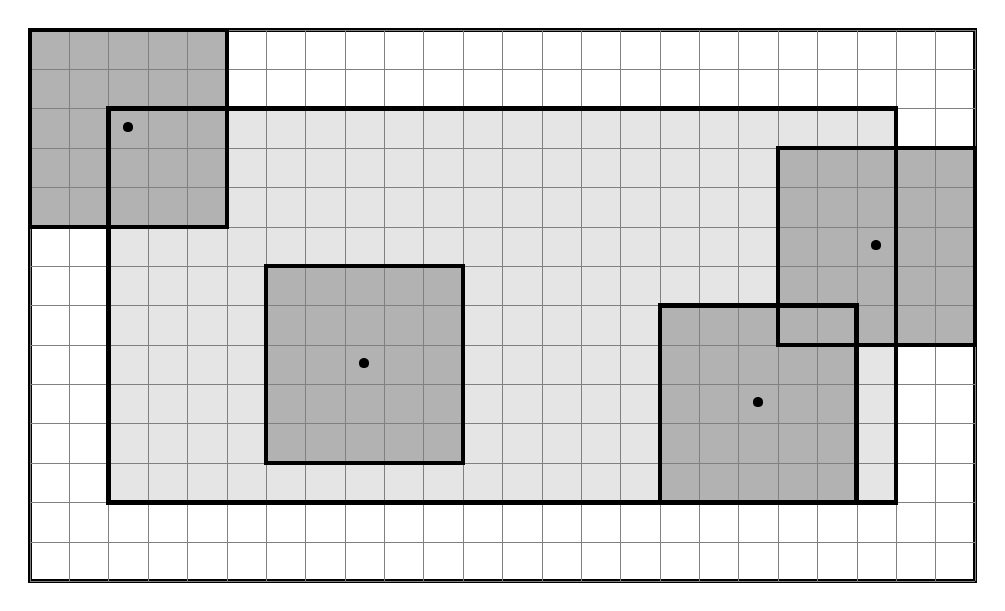
\begin{tikzpicture}
\node[draw, minimum width=12cm, minimum height=
    7cm, ultra thick](outer_rec)[]{};
\node[draw, minimum width=10cm, minimum height=
    5cm, ultra thick, fill=black!10!](inner_rec)[]{};
\node[draw, minimum width=2.5cm, minimum height=2.5cm,
    ultra thick, fill=black!30!](square1)at(-4.75,2.25){\textbullet};
\node[draw, minimum width=2.5cm, minimum height=2.5cm,
    ultra thick,fill=black!30!](square2)at(-1.75,-.75){\textbullet};
\node[draw, minimum width=2.5cm, minimum height=2.5cm,
    ultra thick, fill=black!30!](square3)at(4.75,.75){\textbullet};
\node[draw, minimum width=2.5cm, minimum height=2.5cm,
    ultra thick, fill=black!30!](square4)at(3.25,-1.25){\textbullet};
\draw[step=.5, ultra thin, color=black!50!](-6,-3.5)grid(6,3.5);

\node[draw, minimum width=10cm, minimum height=
    5cm, ultra thick, ][]{};
\node[draw, minimum width=2.5cm, minimum height=2.5cm,
    ultra thick]at(-4.75,2.25){};
\node[draw, minimum width=2.5cm, minimum height=2.5cm,
    ultra thick]at(-1.75,-.75){};
\node[draw, minimum width=2.5cm, minimum height=2.5cm,
    ultra thick]at(4.75,.75){};
\node[draw, minimum width=2.5cm, minimum height=2.5cm,
    ultra thick]at(3.25,-1.25){};
\end{tikzpicture}
\caption{This diagram illustrates how to convolve an image with a filter.
The light grey rectangle represents the original image $A$, and the dark grey squares are the filter $F$.
The larger rectangle is the image padded with zeros; i.e., all pixel values in the outer white band are 0.
To compute the entry of the convolution matrix $C$ located at a black dot, take the inner product of $F$ with the submatrix of the padded image centered at the dot.}
\label{fig:convolution}
\end{figure}

\subsubsection*{Implementation in NumPy} % - - - - - - - - - - - - - - - - - -

Let us write a function that convolves an image with a filter.
You can test this function on the image \li{cameraman.jpg}, which appears in Figure \ref{fig:cameraman}.
The following code loads this image and plots it with matplotlib.

\begin{lstlisting}
>>> image = plt.imread('cameraman.jpg')
>>> plt.imshow(image, cmap = 'gray')
>>> plt.show()
\end{lstlisting}

Here is the function definition and some setup.

\begin{lstlisting}
1. def Filter(image, F):
2.     m, n = image.shape
3.     h, k = F.shape
\end{lstlisting}

To convolve \li{image} with the filter \li{F}, we must first \emph{pad} the array \li{image} with zeros around the edges.
This is because in \eqref{equ:convolve}, entries $A_{ij}$ are set to zero when $i$ or $j$ is out of bounds.
We do this by creating a larger array of zeros, and then making the interior part of the array equal to the original image (see Figure \ref{fig:convolution}).

For example, if the filter is a $3 \times 3$ matrix, then the following code will pad the matrix with the appropriate number of zeros.

\begin{lstlisting}
 # Create a larger matrix of zeros
image_pad = np.zeros((m+2, n+2))
# Make the interior of image_pad equal to the original image
image_pad[1:1+m, 1:1+n] = image
\end{lstlisting}

We want to do this in general in our function.  Note that the number of zeros we need to pad our array depends on the size of the filter \li{F}.

\begin{lstlisting}
5.    image_pad = # Create an array of zeros of the appropriate size
6.   # Make the interior of image_pad equal to image
\end{lstlisting}

Finally, we iterate through the image to compute each entry of the convolution matrix.

\begin{lstlisting}
7.    C = np.zeros(image.shape)
8.    for i in range(m):
9.        for j in range(n):
10.            C[i,j] = # Compute C[i, j]
\end{lstlisting}

\subsubsection*{Gaussian Blur} % - - - - - - - - - - - - - - - - - - - - - - -

A \emph{Gaussian blur} is an image filter that operates on an image by convolving with the matrix
\[
G = \frac{1}{159}\begin{pmatrix}
2&4&5&4&2\\
4&9&12&9&4\\
5&12&15&12&5\\
4&9&12&9&4\\
2&4&5&4&2
\end{pmatrix}.
\]

Blurring an image can remove ``noise'', or random variation that is the visual analog of static in a radio signal (and equally undesirable).

\begin{problem}\label{prob:filter}
\leavevmode
Finish writing the function \li{Filter} by filling in lines 5, 6, and 10.  Hint: Note in \ref{equ:convolve}, $C_{ij}$ was calculated by summing from -1 to 1.  This is only the case if the filter \li{F} is $3 \times 3$. A slight modification is needed in the general case.  Test your function on the image \li{cameraman.jpg} using the Gaussian Blur. The result is in Figure \ref{fig:cameraman_blur}.
\end{problem}

\begin{figure}
\centering
\begin{subfigure}[b]{.49\textwidth}
\centering
\includegraphics[width=\textwidth]{figures/cameraman.jpg}
\caption{Unfiltered image.}
\label{fig:cameraman}
\end{subfigure}
\begin{subfigure}[b]{.49\textwidth}
\centering
\includegraphics[width=\textwidth]{figures/cameramanBlur.pdf}
\caption{Image after Gaussian blur is applied.}
\label{fig:cameraman_blur}
\end{subfigure}
\begin{subfigure}[b]{.49\textwidth}
\centering
\includegraphics[width=\textwidth]{figures/edges.pdf}
\caption{Image after the Sobel filter is applied.}
\label{fig:cameraman_edges}
\end{subfigure}
\caption{Here is an example of a Gaussian blur and the Sobel filter applied to an image.
This photo, known as ``cameraman,'' is a standard test image in image processing.
A database of such images can be downloaded from \url{http://www.imageprocessingplace.com/root_files_V3/image_databases.htm}.}
\label{fig:cameraman1}
\end{figure}

\subsection*{Edge Detection} % ------------------------------------------------

Automatic detection of edges in an image can be used to segment or sharpen the image.
We will find edges with the Sobel filter, which computes the gradient of the image at each pixel.
The magnitude of the gradient tells us the rate of change of the pixel values, and so large magnitudes should
correspond to edges within the image.
The Sobel filter is not a convolution, although it does use convolutions.

We can think of an image as a function from a $2 \times 2$ grid of points to $\mathbb{R}$.
The image maps a pixel location to an intensity.
It does not make sense to define the derivative of this function as a limit because the domain is discrete---a step size $h$ cannot take on arbitrarily small values.
Instead, we \emph{define} the derivative to be the centered difference quotient of the previous section.
That is, we define the derivative in the $x$-direction at the $ij^{th}$ pixel to be
\[
\frac{1}{2}A_{i+1, j} - \frac{1}{2}A_{i-1, j}.
\]

We can use a convolution to create a matrix $A_x$ whose $ij^{th}$ entry is the derivative of $A$ at the $ij^{th}$ entry, in the $x$-direction.
In fact, $A_x = A \ast S$, where
\[
S = \frac{1}{8}
\left[\begin{array}{ccc}
-1 & 0 & 1\\
-2 & 0 & 2\\
-1 & 0 & 1
\end{array}\right].
\]

Note that this convolution takes a weighted average of the $x$-derivatives at $(i, j)$, $(i, j+1)$, and $(i, j-1)$.
The derivative at $(i, j)$ is weighted by 2.
Using a weighted average instead of just the derivative at $(i, j)$ makes the derivative less affected by noise.

Now we can define the Sobel filter.
A Sobel filter applied to an image $A$ results in an array $B = (B_{ij})$ of 0's and 1's, where the 1's trace out the edges in the image.
By definition,
\[
B_{ij} = \left\{
     \begin{array}{ll}
       1 & \text{if}\; \;\|\nabla A(ij)\|_2 > M \\
       0 & \text{otherwise}.
     \end{array}
   \right.
\]
Here, $\nabla A(ij) = ((A \ast S)_{ij}, (A\ast S^T)_{ij})$ is the gradient of $A$ at the $ij^{th}$ pixel.
The constant $M$ should be ``sufficiently large'' enough to pick out those pixels with the largest gradient (i.e., those pixels that are part of an edge).
A good choice for $M$ is 4 times the average value of $\|\nabla A(ij)\|_2$ over the whole image $A$.

When the Sobel filter is applied to \li{cameraman.jpg}, we get the image in Figure \ref{fig:cameraman_edges}.
Here, the 1's in $B$ were mapped to ``white'' and the 0's were mapped to ``black.''

\begin{problem}
Write a function that accepts an image as input and applies the Sobel filter to the image.  Test your function on \li{cameraman.jpg}.  Hint: If you want to find the average of a matrix \li{A}, use the function \li{A.mean()}.
\end{problem}

\end{comment}

